We perform a total training time comparison between TensorFlow implementations and the FPGA hardware. Additionally, we perform a loss convergence comparison between the simulated hardware in MATLAB and the TensorFlow implementation.

\subsection{Total Runtime Results}
After designing the hardware, we simulated the Verilog in Vivado to find the total number of clock cycles to train one batch of mini-batch SGD. We the multiply this value by the operating clock period of the FPGA to determine to absolute time measurement to train a single batch for various clock frequencies. Lastly, we multiply that value by the total number of batches to find the total training time for the given FPGA implementation.

Fig. \ref{fig:total-runtime-plot} displays a comparison of the total training time in minutes between the TensorFlow implementations and the FPGA implementation at varying clock frequencies. As can be seen in the plot, the FPGA needs to be run at 50 MHz minimum to notice any speed up.
\begin{figure}[ht]
	\centering
	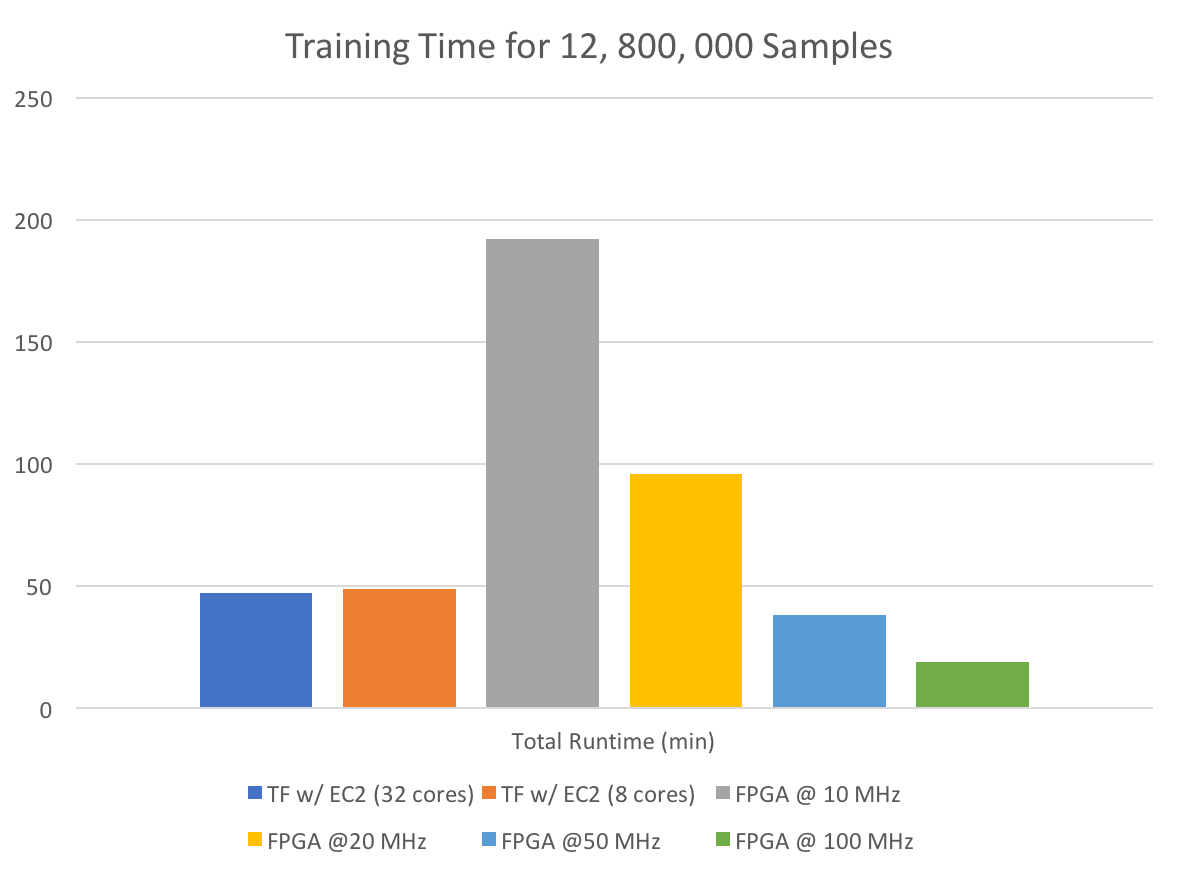
\includegraphics[scale=0.6]{total_runtime_plot.png}
	\caption{A comparison of training time for 12,800,000 samples}
	\label{fig:total-runtime-plot}
\end{figure}

Notice that the TensorFlow implementation notices little to no speed-up going from 8 to 32 cores. This illustrates the lack of potential in current traditional strategies for achieving speed-up by increasing the number of cores or machines. The FPGA implementation, however, scales linearly with frequency. The largest deterrent of running the FPGAs at 100 MHz or higher, is the lack of on-chip resources. Specifically, attempting to fit an entire CNN on a single FPGA introduces too much global routing overhead, which leads to a lower maximum clock frequency. We suspect that by partitioning the neural network by layers onto multiple FPGAs, the hardware will be able to run at the higher frequencies required to achieve speed-up.

\subsection{Loss Convergence Results}
We trained the MATLAB simulation of the hardware using the same dataset as the TensorFlow implementation to verify its convergence. Fig. \ref{fig:loss-plot} illustrates the convergence of the loss versus number of samples processed. Clearly, the loss converges, but it coverges to a worse loss than the full precision TensorFlow implementation.
\begin{figure}[ht]
	\centering
	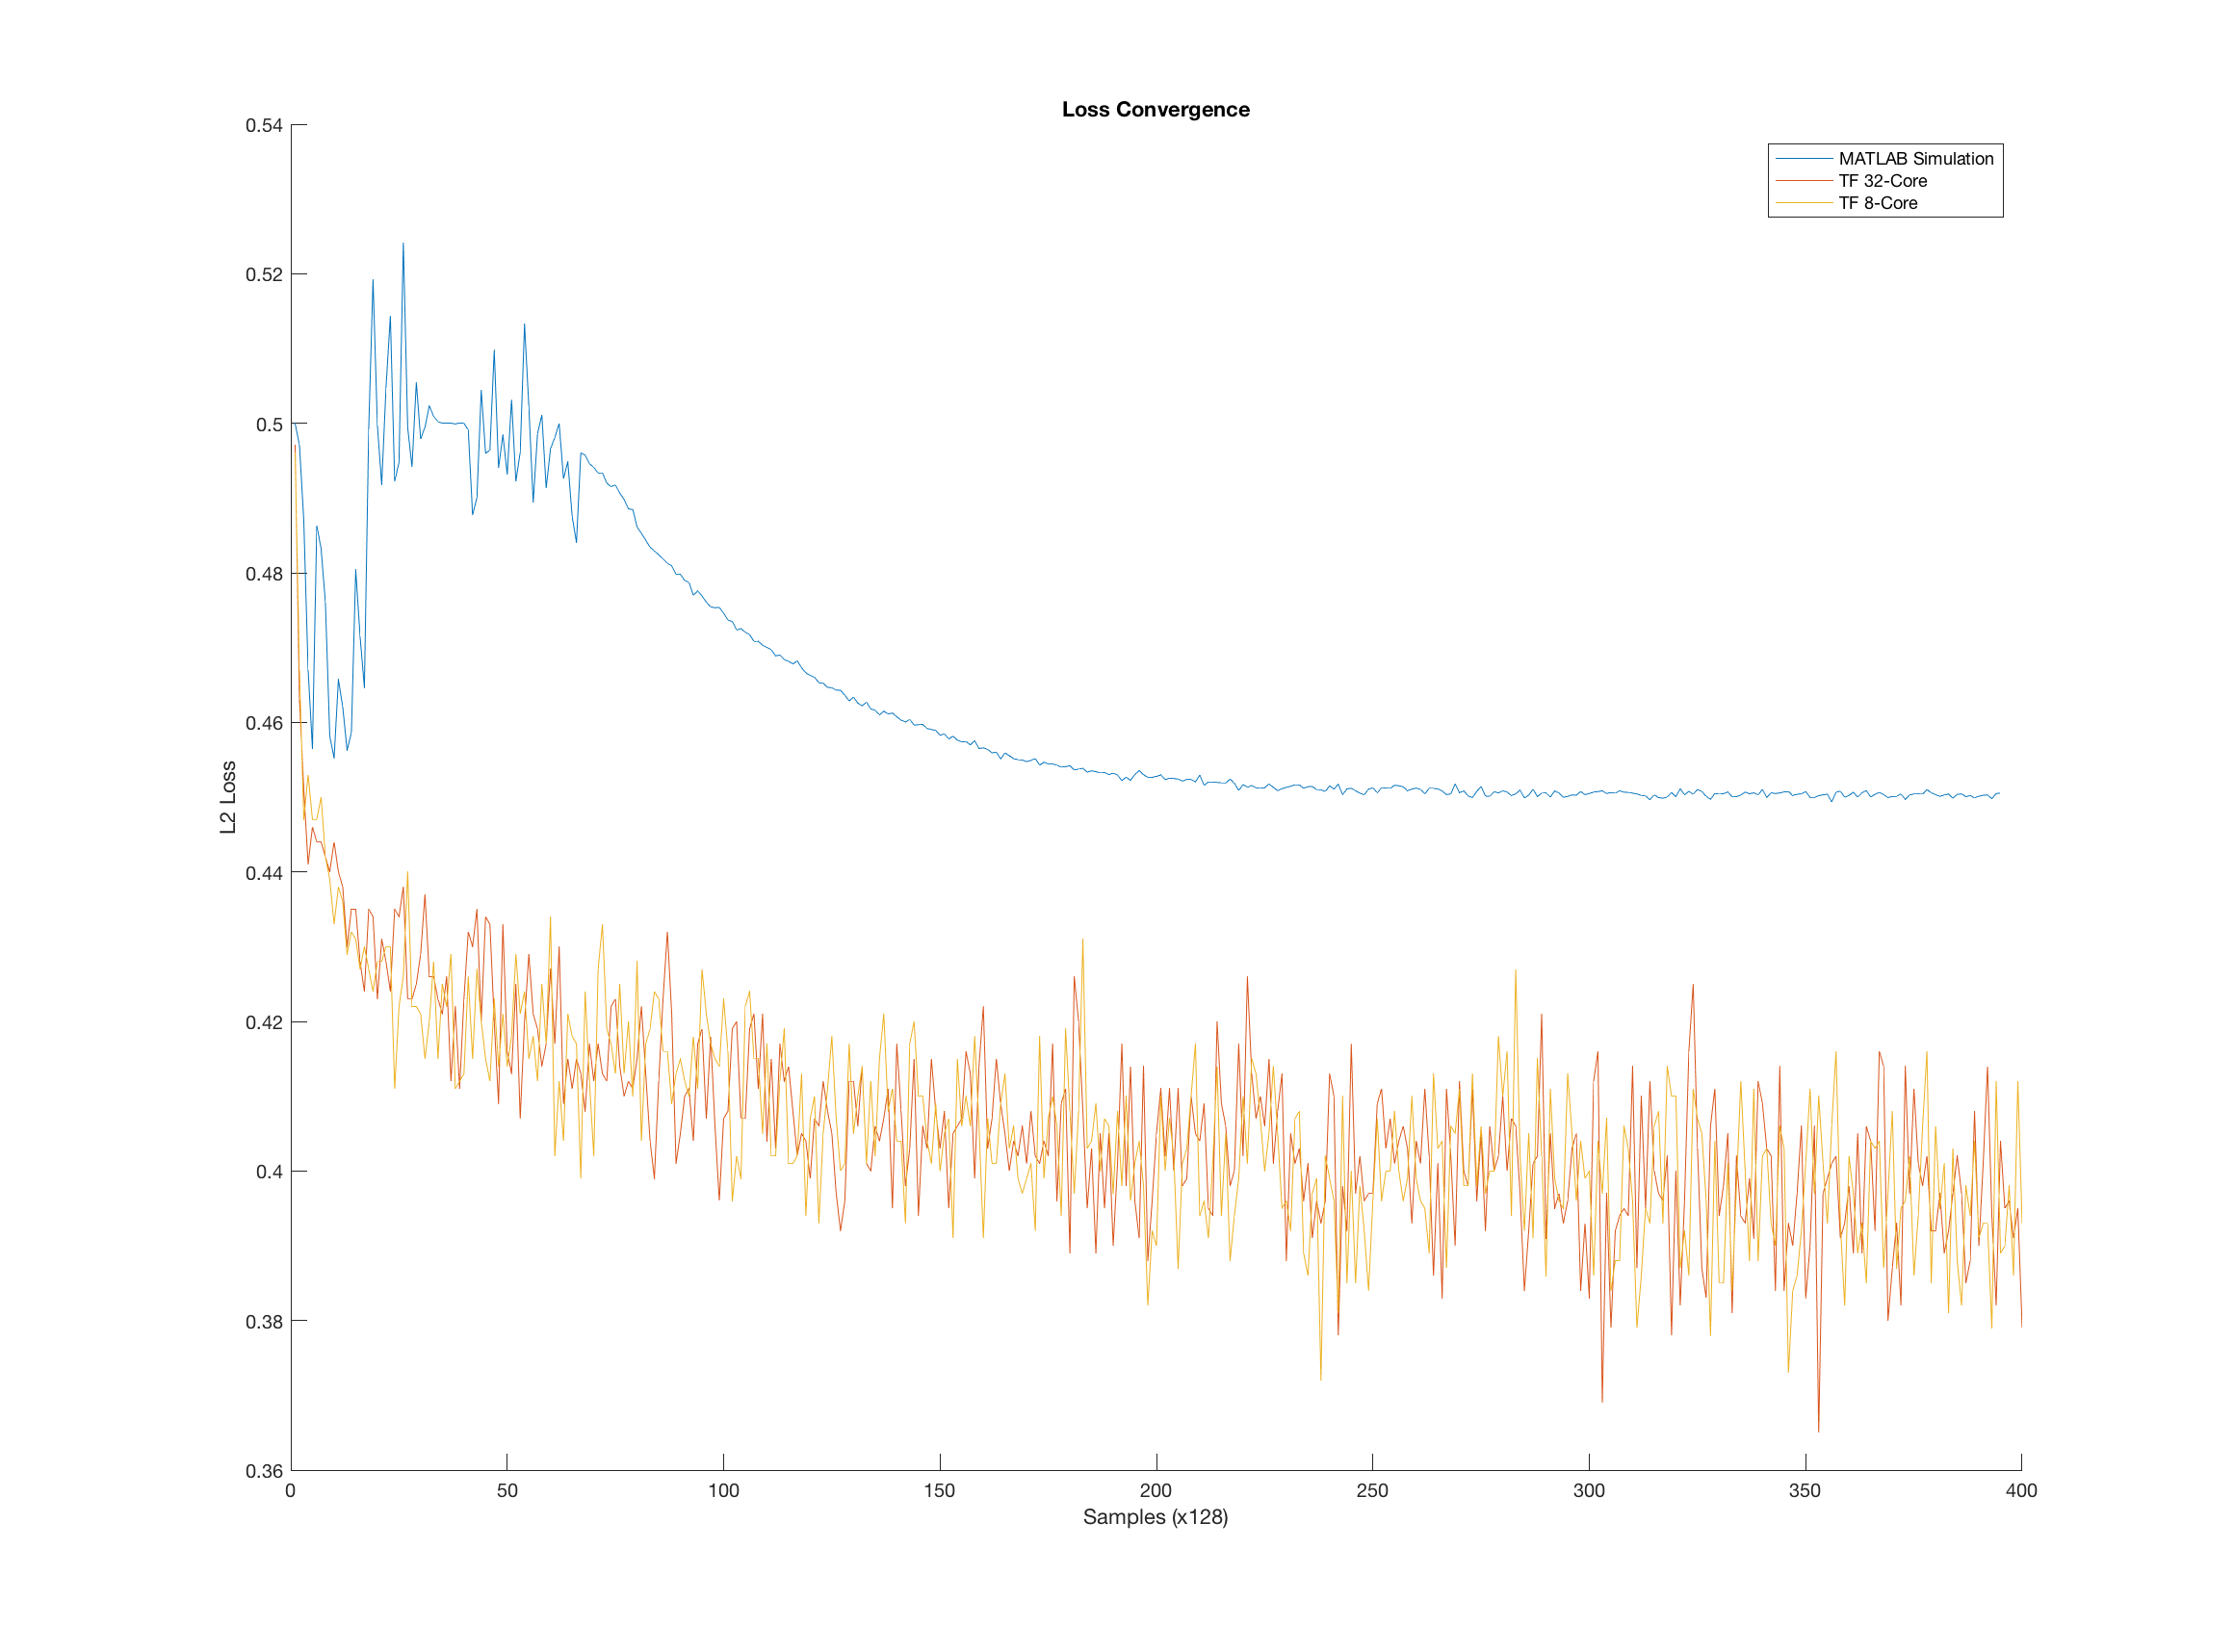
\includegraphics[scale=0.17]{../all_loss_plot.png}
	\caption{The loss versus number of samples processed for the MATLAB and TensorFlow implementations}
	\label{fig:loss-plot}
\end{figure}
The purpose of this analysis was primarily to verify that the hardware is capable of producing a trained CNN. Initially, we expected our loss convergence plots to look similar to Gupta et al. \cite{limited-precision}. However, our plot shows a noticeable difference in the loss value that each implementation converges to. We expect that this is due to the difference in size between our network and the networks implemented by Gupta et al. Since our CNN contains siginificantly less layers and learned parameters, the effect of losing a bit of precision is amplified. In a larger network, the layers can work together to mitigate the effects of losing precision. We believe this discrepancy in the loss convergence plots lends creedence to the need to explore the effects of limited precision training more in depth.